\documentclass[12pt]{article}
\usepackage{fullpage}
\usepackage{natbib}

\usepackage{hyperref}
\hypersetup{colorlinks=true,citecolor=black,urlcolor=blue}

\usepackage{times}

\usepackage{graphicx}
\usepackage{float}
\usepackage{capt-of}
\usepackage{subcaption}

\begin{document}
\title{Reflection Space Image Based Environment Mapping}
\author{Kyung yul Kevin Lim, Myron Liu}
\date{\today}
\maketitle

\section{Abstract}
We implement Reflection Space Image Based Rendering as described by Cabral et al.\cite{cabral1999reflection}. The goal is to generate a scene in which the user can rotate around the object lit by an HDR environment map, and observe view dependent BRDF changes in real time. Possible extensions would be to implement environment maps prefiltering with spherical harmonics for comparison \cite{ramamoorthi2001efficient}.


\section{Milestone Report}

Our focus so far has been to setup the architecture from which we can interact with our shaded geometry in a 3D viewer. This is now fully setup and we can interact with our camera to move around the world and add objects to our scene easily.

Right now we are working primarily on shading a perfectly reflective sphere. We have built a GLSL shader for grabbing the camera position per vertex, and along with the position and normal, compute the reflection direction in spherical coordinates $(\theta,\phi)$. We use RADIANCE HDR maps that are already in latitude longitude panoramic format from \href{http://gl.ict.usc.edu/Data/HighResProbes/}{USC's High-Resolution Light Probe Image Gallery} which makes the conversion straightforward.

Regarding shading diffuse surfaces, we have setup a shader for integrating the environment map over a hemisphere oriented along the surface normal. We naively shaded the sphere using a uniform light source, but soon, we will swap this out for light coming in from every direction, as is the case with environment maps.

Our next steps are to implement the prefiltering and warping of the environment maps which will be headed by Kevin, and continue working on the shader so that we can integrate over the full environment map which will be headed by Myron.


\section{Results}
\begin{figure}[H]
\centering
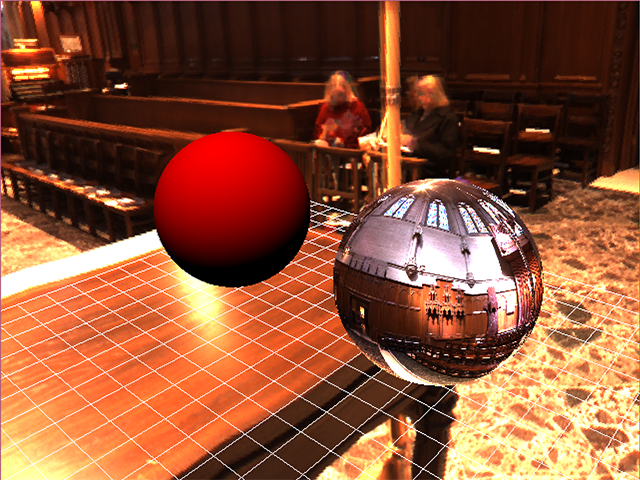
\includegraphics[width=0.75\textwidth]{{Figures/Milestone.png}}
\caption{A diffuse sphere and a fully mirrored sphere} 
\label{fig:milestone}
\end{figure}


\bibliographystyle{plain}
\bibliography{MilestoneReport}

\end{document}

